\setcounter{chapter}{1} 
\chapter{Theoretical Background: the Chemistry of the Arctic Troposphere} \label{ch:theoretical_back}

This chapter provides the background theory for the thesis. It concerns the chemistry of ozone, the impact on the radiative balance, and the heterogeneous reactions causing the depletion of ozone in the troposphere. Further, some of the sources of halogens as well as the mechanisms behind the halogen explosions are investigated. 

\begin{figure}
    \centering
    \includegraphics[width = 0.6\linewidth]{Chapter2_Theory/images/sea_ice.JPG}
    \caption{Sea ice in St. Jonsfjorden, Svalbard on 22 April at 23:00 UTC, 2018 (photograph: Private)}
    \label{fig:sea_ice}
\end{figure}


\section{Atmospheric radiation}\label{sec:atm_rad}

The Earth's energy balance is the balance between the incoming shortwave radiation from the Sun and the \acrfull{olr} that the Earth emits to space. The average temperature on Earth is fairly constant. Thus, radiant energy from the sun that is absorbed by the earth-atmosphere system must be re-emitted in order for the equilibrium energy state to be maintained. The emitted energy from the Earth is referred to as thermal \acrfull{ir} (\cite{Liou_AtmRad}, \cite{SeinfeldSpyros}). 

\medskip

Any imbalance occurring in the the Earth-atmosphere system due to external agents is quantified as the \acrfull{rf} (\cite{IPCCchapter8}, \cite{Bowman2013}). RF is usually expressed in watts per square meter over a particular period of time, such as pre-industrial to present day (\cite{IPCCchapter8}). The estimated RF change due to tropospheric $\chem{O_3}$ since pre-industrial times is estimated to be 0.40 (0.20 to 0.60) Wm$^{-2}$ (\cite{IPCCchapter8}). 


\medskip

Photodissociation of a molecule can occur when the energy of the photon exceeds the binding energy between the molecule's components (\cite{SeinfeldSpyros}). The photodissociation of ozone: $\chem{O_3} + hv \rightarrow \chem{O_2} + \chem{O}$, can yield various electronic states of the products \chem{O} and $\chem{O_2}$ depending on the wavelength of the incident radiation, with the singlet-D oxygen atom, $\chem{O}(^1\chem{D})$ being the most important electronically excited species of the atmosphere as it's reaction with water vapor is a source of \chem{OH} radicals, enhancing the oxidation capacity of the atmosphere (\cite{SeinfeldSpyros}).


\medskip

The absorption spectra of ozone is varying according to the strength of the chemical bands in the molecule. The strongest band (Hartley band - $\chem{O(^3P)}$ formation) absorbs highly energetic \acrfull{uv} radiation from the sun in the upper stratosphere and mesosphere in the wavelength range 242-310 nm. The UV Absorption spectrum of $\chem{O_2}$ is strongly connected to the formation of ozone, and absorbs in the range of 100-242 nm in the thermosphere, mesosphere and stratosphere. At about 50 km altitude, the maximum ozone absorption occurs in the Hartley band. In the lower stratosphere and troposphere, ozone absorbs solar flux in the range 310-400 nm (Huggins bands - $\chem{O(^3P)}$ formation). The weakest band (Chappuis bands) absorbs in the visible- and near IR region in the troposphere. The absorption range is 400-850 nm (\cite{Liou_AtmRad}). 



\medskip 

In the thermal infrared, ozone absorbs in two main bands, which are in the 9.6 and 14.27 $\mu$m regions. The latter band is overlapped by the $\chem{CO_2}$ 15 $\mu$m band. The atmospheric window is the wavelength range in which the atmosphere is relatively transparent. Thus, most IR absorption occurs outside the wavelength region 8-12 $\mu$m (\cite{AtmModFund}), which makes the 9.6 band the most important absorption band for ozone (\cite{Liou_AtmRad}, \cite{Myhre1997}). Due to it's absorption in the IR region, ozone is a gas that contributes to the greenhouse effect, i.e. it contributes to the trapping of thermal IR, and thus heating of the atmosphere (\cite{Liou_AtmRad}).



\section{Ozone and its precursors}\label{sec:ozone_and_precursors}

Ozone is a colorless gas that impacts the life on our planet in different ways, depending on the location of it's occurrence. If situated in the stratosphere (the ozone layer) it absorbs harmful UV radiation from the Sun in the range of 100-315 nm, and is thus essentially functioning as a shield for the planet (\cite{SeinfeldSpyros}). However, if located in the lower troposphere, ozone affects human health and vegetation. Concentrations above 0.1 \acrfull{ppm} interferes with the growth of plants, and has unhealthy impacts on humans (\cite{AtmModFund}). Typical concentrations in the free troposphere range from 20 to 40 \acrfull{ppb} near sea level and from 30 to 70 ppb at higher altitudes. In moderately to severely polluted urban areas, concentrations may range from 0.01 ppm to 0.35 ppm (\cite{AtmModFund}).  

\medskip

Stratospheric ozone has a natural origin, resulting from the photolytical decomposition of $\chem{O_2}$ followed by the oxygen atom reacting with another $\chem{O_2}$ molecule, thus producing two $\chem{O_3}$ molecules. The ozone molecules themselves may continue to react with other anthropogenic and/or naturally occurring stratospheric molecules. Generally, the concentration of $\chem{O_3}$ in the stratosphere is in steady-state due to the balance of it's production and destruction, and at the peak of the ozone layer, the $\chem{O_3}$ mixing ratio is about 12 ppm (\cite{SeinfeldSpyros}).  

\medskip

In the troposphere, ozone is a secondary pollutant resulting from two major classes of precursors; volatile organic compounds (VOCs) and oxides of nitrogen ($\chem{NO_x} = \chem{NO} + \chem{NO_2}$). In urban areas, $\chem{NO_x}$ mixing ratios range from 5 to 20 ppb. In rural areas, concentrations are about 1 ppb, and in remote areas, concentrations range from 10 to 100 ppt. In remote areas, ozone formation is sustained by $\chem{CH_4}$ and \chem{CO} through reactions with \chem{OH} (\cite{Cadle1970}, \cite{Levy1971}, \cite{SeinfeldSpyros}). The production of ozone is thus usually limited by the access of $\chem{NO_x}$ and $\chem{HO_x} (\chem{HO} + \chem{HO_2})$ (\cite{Levy1971}). The main removal pathways in the troposphere are through photolysis and through reaction with $\chem{HO_2}$ (\cite{SeinfeldSpyros}).

\medskip

One of the features of the stable Arctic boundary layer is the Arctic front. The front acts as a transport barrier that isolates the Arctic lower troposphere towards lower latitudes (\cite{BARRIE1986643}). In order to transport polluted air to the Arctic lower troposphere on a timescale of a few weeks, the source region of the pollution must be cold enough as well as located north of the Arctic front, which may extend down to about 40 $^o$N in January (\cite{BARRIE1986643}, \cite{AMAP2015}). 


\medskip

Both in the troposphere and the stratosphere, the $\chem{O_3}$ photolysis occurs, which produces both ground-state \chem{O} and excited singlet $\chem{O(^1D)}$ oxygen atoms (\cite{SeinfeldSpyros}): 

\begin{reaction}
    \chem{O_3} + hv \rightarrow \chem{O_2} + \chem{O}
    \label{rqn:groundstate_O2}
\end{reaction}

\begin{reaction}
    \chem{O_3} + hv \rightarrow \chem{O_2} + \chem{O(^1D)}
    \label{rqn:excited_O2}
\end{reaction}

The ground-state oxygen atom rapidly reacts with an oxygen molecule to re-form ozone, thus forming a null-cycle:

\begin{reaction}
    \chem{O} + \chem{O_2} + \chem{M} \rightarrow \chem{O_3} + \chem{M}
    \label{rqn:ozone}
\end{reaction}

Reaction \ref{rqn:ozone} is the most significant source of ozone in the atmosphere (\cite{SeinfeldSpyros}). The excited oxygen atom, however must react with another atmospheric species to rid itself from excess energy. Most often, it collides with $\chem{N_2}$ or $\chem{O_2}$, which removes the excess energy, quenching it back to it's ground state (\cite{Levy1971}). Every now and then, however, the excited oxygen atom may react with $\chem{H_2O}$ to form \chem{OH} radicals (\cite{SeinfeldSpyros}): 

\begin{reaction}
    \chem{O(^1D)} + \chem{H_2O} \rightarrow 2\chem{OH}
    \label{rqn:OH}
\end{reaction}

This is the only gas-phase reaction in the troposphere that is able to break the \chem{H-O} bond in $\chem{H_2O}$ (\cite{SeinfeldSpyros}). Tropospheric ozone is thus increasing the oxidizing capacity of the troposphere as it is acting as a precursor for \chem{OH}. The hydroxyl radicals interplay in a chain of reaction that results in the removal of atmospheric \chem{CO} and $\chem{CH_4}$ (\cite{Levy1971}). 

\medskip

When \chem{NO} and $\chem{NO_2}$ is present in sunlight, ozone may be produced photochemically (i.e. the initiating step is the absorption of a photon (\cite{Cadle1970})) in by the photolysis of $\chem{NO_2}$ (Reaction \ref{rqn:no2hv} below) followed by Reaction \ref{rqn:ozone} (\cite{Hesstvedt1978}): 


\begin{reaction}
    \chem{NO_2} + hv \rightarrow \chem{O} + \chem{NO}
    \label{rqn:no2hv}
\end{reaction}

The \chem{NO}-molecule quickly reacts with ozone to regenerate $\chem{NO_2}$:


\begin{reaction}
    \chem{O_3} + \chem{NO} \rightarrow \chem{O_2} + \chem{NO_2}
    \label{rqn:o3no}
\end{reaction}




\section{Halogen chemistry}\label{sec:halogen_chemistry}


The halogens are a group in the periodic table consisting of fluorine, chlorine, bromine and iodine, as well as astatine, which is incredibly rare and therefore not considered to be of importance in the case of ozone depletion caused by reactive halogens. Natural occurrence of halogens and halogen-containing compounds can be found in sea water (as well as other sources, which will not be considered here). The halogens that pay partake in ozone depletion occur in the following abundance (more abundant to less abundant); chloride, bromide and iodide (\cite{Simpson2015}). 

\medskip

Even though bromide is less abundant than chloride, it is most prone to participate in the depletion of ozone. The reason for this is that chlorine has a similar bond strength with hydrogen as it has with hydrocarbons (such as methane), and is therefore prone to react with hydrocarbons rather than act to deplete ozone: 

\begin{reaction}
    \chem{Cl} + \chem{CH_4} \rightarrow \chem{HCl} + \chem{CH_3}
    \label{R:cl_ch4}
\end{reaction}

In a field study at Alert conducted by \cite{Foster2001}, they found $\chem{Br_2}$ and \chem{BrCl} molecules in relation with \acrshort{ode}. $\chem{Cl_2}$ on the other hand, was below the detection limit throughout the measuring period, indicating that the chlorine compound that is active in the ODEs is \chem{BrCl}- 

\medskip

Bromine, on the other hand, is less reactive towards hydrocarbons and readily depletes ozone in a catalytic manner.  Fluorine creates strong bonds with hydrogen, and is thus not reactive towards ozone. Aqueous iodine is less abundant than bromine and chlorine in the ocean due to it's role as a nutrient for biological systems (\cite{FinlaysonPitts2010}, \cite{Simpson2015}). 

\medskip

Thus, the focus in this thesis will be bromide, and to some extent chlorine reactive species. The reactive halogens have short lifetimes on the order of seconds to minutes and are typically only present during the day as they are activated by photolysis:



\begin{reaction}
    \chem{BrCl} + hv \rightarrow \chem{Br} + \chem{Cl}
    \label{R:19}
\end{reaction}

\begin{reaction}
    \chem{Br_2} + hv \rightarrow 2\chem{Br}
\end{reaction}

Throughout this and the following section, halogen species which partake in ozone depletion will be denoted as "\chem{X}". Reactive halogens denotes radical species such as atomic halogen species, \chem{X}, and their higher oxides, \chem{XO}. 

\begin{reaction}
    \chem{X_2} + hv \rightarrow 2\chem{X} \label{R:1}
\end{reaction}

The absorption spectra of dihalogens lies in the actinic (visible to near-UV) part of the spectra. Thus, photolysis may occur at longer wavelengths than that of ozone photochemistry, which requires UV photons near 300 nm (Photolysis of ozone is highly dependent on ozone column at higher altitudes, see Section \ref{sec:atm_rad}) (\cite{Simpson2015}).

\medskip

Halogen reservoir species are nonradicals that sequester reactive halogens. These include species such as $\chem{X_2}$, $\chem{HOX}$, $\chem{XONO_2}$ and $\chem{HX}$. The halogen reservoir species are less reactive, and hence the lifetime of theirs are longer than the reactive species (\cite{Simpson2015}). Moreover, \cite{Foster2001} found that $\chem{Br_2}$ and \chem{BrCl} were produced in high amounts at the time when polar sunrise occurred. This may point to a build-up of photolabile halogen species during the polar night. A similar theory was suggested by Simpson et.al. (\cite{Simpson2018}) who found that peak \chem{BrO} concentrations were found in airmasses that had been exposed to minimal photolysis of $\chem{Br_2}$ (Utquiavik (Barrow), Alaska). More information about halogen sources can be found in Section \ref{sec:halogen_sources}. 



\subsection{Bromine explosion}\label{sec:BE}

The discovery of ODEs in the troposphere due to anomalously high concentrations of reactive halogen species, bromine in particular, was made by Barrie and coworkers at Alert in Canada in 186-1987 (\cite{BARRIE1986643}). Ozone depletion was a well known phenomena at this point, but was unexplained until then (e.g. \cite{Oltmans1981}). 

\medskip

During polar spring, the amount of ozone in the polar boundary layer may decrease from tens of ppb to less than 1 ppb due to catalytic destruction by reactive halogen species (\cite{CAO}). the reaction scheme assuming bromine is the depleting agent is to a large extent summarized in Figure \ref{fig:het_react}. 

\medskip

\begin{figure}
    \centering
    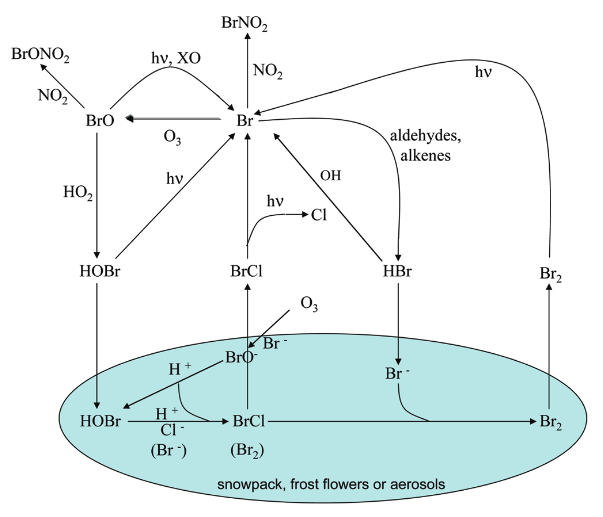
\includegraphics[width=0.7\linewidth]{Chapter2_Theory/images/ODE_Finlayson-Pitts.png}
    \caption{Typical heterogeneous reaction model. The blue shaded area illustrates the condensed phase. Image taken from \cite{FinlaysonPitts2010}}
    \label{fig:het_react}
\end{figure}


The production of halogen radicals and subsequent ozone depletion may proceed as follows (The set of reactions is taken from \cite{CAO} and \cite{Simpson2015}): 

\medskip

Reaction \ref{R:1} produces two halogen radicals, which are highly reactive. Ozone is then destroyed by: 

\begin{reaction}
    \chem{X} + \chem{O_3} \rightarrow \chem{XO} + \chem{O_2}
    \label{R:2}
\end{reaction}

The halogen oxides may proceed to deplete ozone. They partition quickly between the the following reactions and either reactivate by Reaction \ref{R:1}, or becoming radical directly:


\begin{reaction}
    \chem{XO} + \chem{XO} \rightarrow \chem{X_2} + \chem{O_2} \label{R:3} 
\end{reaction}


\begin{reaction}
    \chem{XO} + \chem{XO} \rightarrow \chem{X} + \chem{X} + \chem{O_2} \label{R:4} 
\end{reaction}


\begin{reaction}
    \chem{XO} + \chem{XO} \rightarrow \chem{OXO} + \chem{X} \label{R:5} 
\end{reaction}

The \chem{XO}-self reaction in Reactions \ref{R:3} to \ref{R:5} are often considered the rate limiting step for $\chem{O_3}$ destruction (\cite{JPL}). The partitioning between \chem{XO} and \chem{X} is rapid (\cite{Schmidt} reported a $[\chem{XO}]/[\chem{X}]$ ratio globally close to 1). In addition to the partitioning in Reactions \ref{R:3} to \ref{R:5}, \chem{XO} may be oxidized or photolysed:  

\begin{reaction}
    \chem{OH} + \chem{XO} \rightarrow \chem{X} + \chem{HO_2}
    \label{R:15}
\end{reaction}

\begin{reaction}
    \chem{XO} + hv \rightarrow \chem{X} + \chem{O}
    \label{R:20}
\end{reaction}

The halogen oxides quickly photodissociate (on the order of seconds and minutes time scale) and Reactions \ref{R:2} and \ref{R:20} creates a null cycle that does not destroy or produce ozone. This has an effect on the partitioning of \chem{X} and \chem{XO} species. The oxides dominate the radical form, which extends the lifetime of the $\chem{XO_x} = \chem{X} + \chem{XO}$-family as the oxides are generally less reactive than the atomic form (\cite{Simpson2015}). 

\medskip

Termination reactions that renders the \chem{XO}-radical into the reservoir species \chem{HBr}, \chem{HOBr} and $\chem{BrONO_2}$ may proceed as follows: 

\begin{reaction}
    \chem{XO} + \chem{HO_2} \rightarrow \chem{HOX} + \chem{O_2}
    \label{R:6} 
\end{reaction}

\begin{reaction}
    \chem{X} + \chem{HO_2} \rightarrow \chem{HX} + \chem{O_2}
    \label{R:17}
\end{reaction}


\begin{reaction}
    \chem{OH} + \chem{XO} \rightarrow \chem{HX} + \chem{O_2}
    \label{R:16}
\end{reaction}

\begin{reaction}
    \chem{BrO} + \chem{NO_2} + M \rightarrow \chem{BrONO_2} + M
    \label{R:9}
\end{reaction}

Depending on their relative bond strength, the reservoir species may be reactivated by: 


\begin{reaction}
    \chem{BrO} + \chem{NO} \rightarrow \chem{NO_2} + \chem{Br}
    \label{R:14}
\end{reaction}



\begin{reaction}
    \chem{BrONO_2} + \chem{H_2O} \xrightarrow{aerosol} \chem{HOBr} + \chem{HNO_3}
    \label{R:13}
\end{reaction}

\begin{reaction}
    \chem{HOBr} + hv \rightarrow \chem{Br} + \chem{OH}
    \label{R:18}
\end{reaction}


The bromine explosion events involves reaction \ref{R:1}, \ref{R:2} and \ref{R:6}, with $\chem{X} = \chem{Br}$, in an autocatalytic manner by the means of heterogeneous reactions: 

\begin{reaction}
    \chem{HOBr} + \chem{X^-_{aq}} + \chem{H^+_{aq}} \xrightarrow{snow/ice} \chem{BrX} + \chem{H_2O} \label{R:7} 
\end{reaction}
\begin{reaction}
    \chem{HOBr} + \chem{HX_{aq}} \xrightarrow{aerosol} \chem{BrX} + \chem{H_2O} \label{R:8}
\end{reaction}



In which the multiphase Reactions \ref{R:7} and \ref{R:8} outlines the release of bromine radicals from the condensed phase on snow/ice surfaces or aerosol surfaces, respectively. In this case, \chem{X} may denote \chem{Br} or \chem{Cl}, normally. The full multiphase reaction is dependent on temperature, sunlight and an acidic reaction surface (\cite{Toyota}). The bromine explosion can be summed up as follows: 

\begin{align*}
    \chem{HOBr} + \chem{X^-_{aq}} + \chem{H^+_{aq}} &\xrightarrow{snow/ice} \chem{BrX} + \chem{H_2O} \\
    \chem{Br_2} + hv &\rightarrow 2\chem{Br} \\
    \chem{Br} + \chem{O_3} &\rightarrow \chem{BrO} + \chem{O_2} \\
    \chem{BrO} + \chem{HO_2} &\rightarrow \chem{HOBr} + \chem{O_2} \\
    \text{NET:} \quad \chem{X^-_{aq}} + \chem{H^+_{aq}} + \chem{HO_2} + \chem{O_3}  &\rightarrow \chem{Br} + \chem{H_2O} + 2\chem{O_2} 
\end{align*}

\medskip

The reactive surface maybe supplied by different media, and this is an object of many research articles (e.g.  \cite{Simpson2018}, \cite{Rankin}). Whichever is more significant, there is most likely a cooperation of the reactive surfaces that accelerates the bromine explosion events. The reactive surfaces are (generally): 

\begin{itemize}
    \item Newly formed sea ice: Has a higher salinity and a higher bromine content than old sea ice and sea water \cite{Rankin}
    \item Snow surfaces, with low pH
    \item Aerosol surfaces, with low pH
\end{itemize}

\subsubsection{Chlorine reservoir species}

In the stratosphere, $\chem{NO_2}$ and $\chem{CH_4}$ are responsible for shifting reactive chlorine species into reservoir species (\cite{SeinfeldSpyros}). Methane acts via Reaction \ref{R:cl_ch4} to form $\chem{CH_3}$. Reservoir compounds may form by the reaction of \chem{XO} and $\chem{NO_2}$: 

\begin{reaction}
    \chem{ClO} + \chem{NO_2} + M \rightarrow \chem{ClONO_2} + M
    \label{R:clono2}
\end{reaction}

\subsection{Halogen sources}\label{sec:halogen_sources}

Sources of reactive halogens in the troposphere include photochemical degradation of organobromines ($\chem{CHBr_3}$, $\chem{CH_2Br_2}$, $\chem{CH_3Br}$), release of bromine from \acrfull{ssa} and transport from the stratosphere (\cite{Schmidt}). 

\medskip

Model studies has shown that the release of reactive halogen species from SSA is particularly relevant in polar regions (\cite{Schmidt}). While SSA is a known and certain source of reactive bromine species in the Arctic, the surface on which sea salt is transformed into gas-phase reactive halogens is somewhat unclear (\cite{Simpson2005}). SSA is formed though the breaking of waves at the ocean surface (\cite{Simpson2015}). 

\medskip

Formation of reactive halogen species though frost flowers has been suggested as a potential source. Frost flowers are ice crystals that forms on new sea ice when air that is supersaturated with water vapor condenses at the surface of the ice (\cite{GRANFORS2013124}, \cite{Kaleschke}). However, the sporadic nature and short lifetime of frost flowers points to other sources that may be more prominent as ODEs occur frequently during the polar spring. Snowpack measurements over coastal- and central Arctic \acrfull{fyi} and remote \acrfull{myi} performed by \cite{Peterson2019} revealed mostly snowpacks enriched in bromide species as a potential source of reactive bromine. This suggests that both MYI and FYI plays a role in the activation of halogens that subsequently may deplete ozone. The halides are incorporated in the snowpack by transported snow containing SSA (\cite{Toyota}, \cite{Peterson2019}). Trace bromine gases, such as \chem{HBr}, \chem{HOBr} and $\chem{BrONO_2}$, may be produced in the snowpack or deposited through mulitphase-reactions (\cite{Simpson2005}). 


\medskip


In the marine boundary layer, chlorine is the most abundant halide and is released from SSA by as $\chem{HCL}$ by acid displacement and photochemically as reactive halogens or their precursors. There is a difference between the marine boundary layer in polar regions and outside polar regions with respect to observed contents of $\chem{BrO}$ and $\chem{BrCl}$. Observations of these species rarely exceed detection limits and in the case of $\chem{BrCl}$, it is hardly observed at all (\cite{Simpson2015}). 

\medskip

The ocean also provides a large source of bromine- and iodide containing halocarbons that, when emitted into the troposphere, comprise very short-lived species (VSLS) that influence ozone destruction both in the troposphere and stratosphere (\cite{ziska}, \cite{Simpson2015}). The most abundant short-lived halocarbon (containing bromine) in the atmosphere and ocean are bromoform ($\chem{CHBr_3}$) and dibromomethane ($\chem{CH_2Br_2}$). Bromoform and dibromomethane is produced by marine organisms such as macroalgae and phytoplankton (\cite{Quack2003}).


\medskip

The oxidation of $\chem{CHBr_3}$ and $\chem{CH_2Br_2}$ as well as the photolysis of $\chem{CHBr_3}$ is applied as a source for tropospheric $\chem{Br_y}$ in this set-up following \cite{Parella}:


\begin{reaction}
    \chem{CHBr_3} + \chem{OH} \rightarrow 3\chem{Br} + \chem{Products}
    \label{R:10}
\end{reaction} 
\begin{reaction}
    \chem{CH_2Br_2} + \chem{OH} \rightarrow 2\chem{Br} + \chem{Products}
    \label{R:11}
\end{reaction}
\begin{reaction}
    \chem{CHBr_3} + hv \rightarrow 3\chem{Br} + \chem{Products}
    \label{R:12}
\end{reaction}

\medskip

Reactive bromine species and their precursors may also be transported, either within the Arctic boundary layer (\cite{Luo2018}, \cite{Schmidt}), or from the stratosphere. 


\subsection{Influence of nitrogen}\label{sec:influence_of_nitrogen}


Generally, tropospheric ozone is a result of two main precursors, $\chem{NO_x} = \chem{NO} + \chem{NO_2}$

In polluted regions, there is an important balance between regions with too much $\chem{NO_x}$, which generally acts as a precursor of ozone, and areas where the $\chem{NO_x}$ concentration is low enough to sustain the production of ozone depleting reactive halogens. The high concentrations of $\chem{HNO_3}$ and $\chem{H_2SO_4}$ can in theory provide the reactive surfaces for acidity dependent autocatalytic release of reactive halogens, but the efficiency of this mechanism is degraded in the case of $\chem{NO_x}$ and hydrocarbon concentrations (\cite{Simpson2015}). High concentrations of $\chem{NO_x}$ suppresses the formation of $\chem{HO_x}$, which is in turn a key component of the halogen explosion sequence. Hydrocarbons serve as sinks for reactive halogens due to their willingness to react with these rather than with ozone, and thus terminates the halogen explosion sequence (\cite{Simpson2015}). Incidents in which halogens do get activated in polluted regions, production of nitryl halides, $\chem{XNO_2}$, is considered to be a major activation process. Observations have shown that this is mostly relevant for chlorine as the reactivity and/or solubility of $\chem{BrNO_2}$ and $\chem{INO_2}$ are likely much greater than for $\chem{ClNO_2}$ \cite{Simpson2015}. 

\medskip





\cite{SeinfeldSpyros} SKRIV OM HIGH NOX/LOW NOX ENVIRONMENTS

In the troposphere, ozone is a secondary pollutant produced in areas with high anthropogenic emissions of $\chem{NO_x}$. 